\section{Introdução e escopo}

\subsection{Contextualização e objetivo}
O sistema que foi projetado consiste em uma unidade de energia composta por dois conjuntos de baterias e um ultracapacitor, conectados a um barramento CC por conversores que operam em modo de condução contínua e uma carga R, como indicado pela imagem \ref{fig:diagrama}.

\begin{figure}[H]
    \centering
    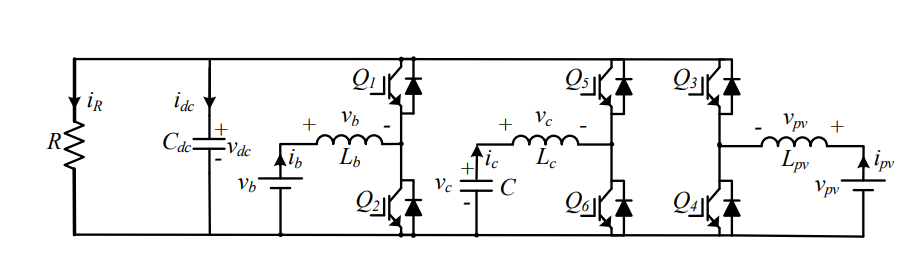
\includegraphics[width=0.5\textwidth]{images/diagrama.png}

    \caption{Diagrama do sistema}
    \label{fig:diagrama}
\end{figure}

Para o chaveamento de cada par de transistores(3 pares), forma implemantados os sinais de PWM, sendo que a condução de um par se comporta de forma complementar entre si, ou seja, quando um transistor está conduzindo, o outro está desligado, tendo ciclos de trabalho de db, dpv e dc, para o par do convesor de bateria de primeira vida, segunda vida e ultracapacitor, respectivamente.

Para o projeto do sistema, deve-se determinar todos os circuitos além dos comportamentos de tensão e corrente sobre LC, e portanto deve projetar os indutores e capacitores para que tenha uma ondulação inverior a 10\% e 20\% da tensaõ em seu respectivo componente para uma determjinada potência.

Após isso, deve-se determinar o modelo de espaço de estados do sistema,validar o sistema com simulações  e então projetar um controlador droop para a malha externa de tensão, com o objetivo de melhorar a resposta do sistema.


Por fim deve-se calcular o comportamento da resposta em frequência da impedância vista pela carga e o comportamento dos autovalores, evidenciando a influência do controle sobre a impedância e sobre a estabilidade.


\subsection{Parâmetros e escopo do projeto}
Foi considerado alguns valores de parâmeteros para o projeto do sistema, indicados pela tabela abaixo:

\begin{table}[H]
    \caption{Parâmetros adotados para o projeto demonstrativo}
    \label{tab:parametros}
    \centering
    \begin{tabular}{llll}
        \toprule
        Grandeza & Valor & Grandeza & Valor \\
        \midrule
        $V_{dc}$                & 400 V          & $V_{c,0}$            & 300 V          \\
        $P_R$                   & 8 kW           &  $V_b$                & 200 V        \\
        $R$                     & 20 $\Omega$    & $V_{pv}$                & 250 V       \\
        $f_s$                   & 20 kHz         & $I_R$                & 20 A           \\
       
        \bottomrule
    \end{tabular}
\end{table}





